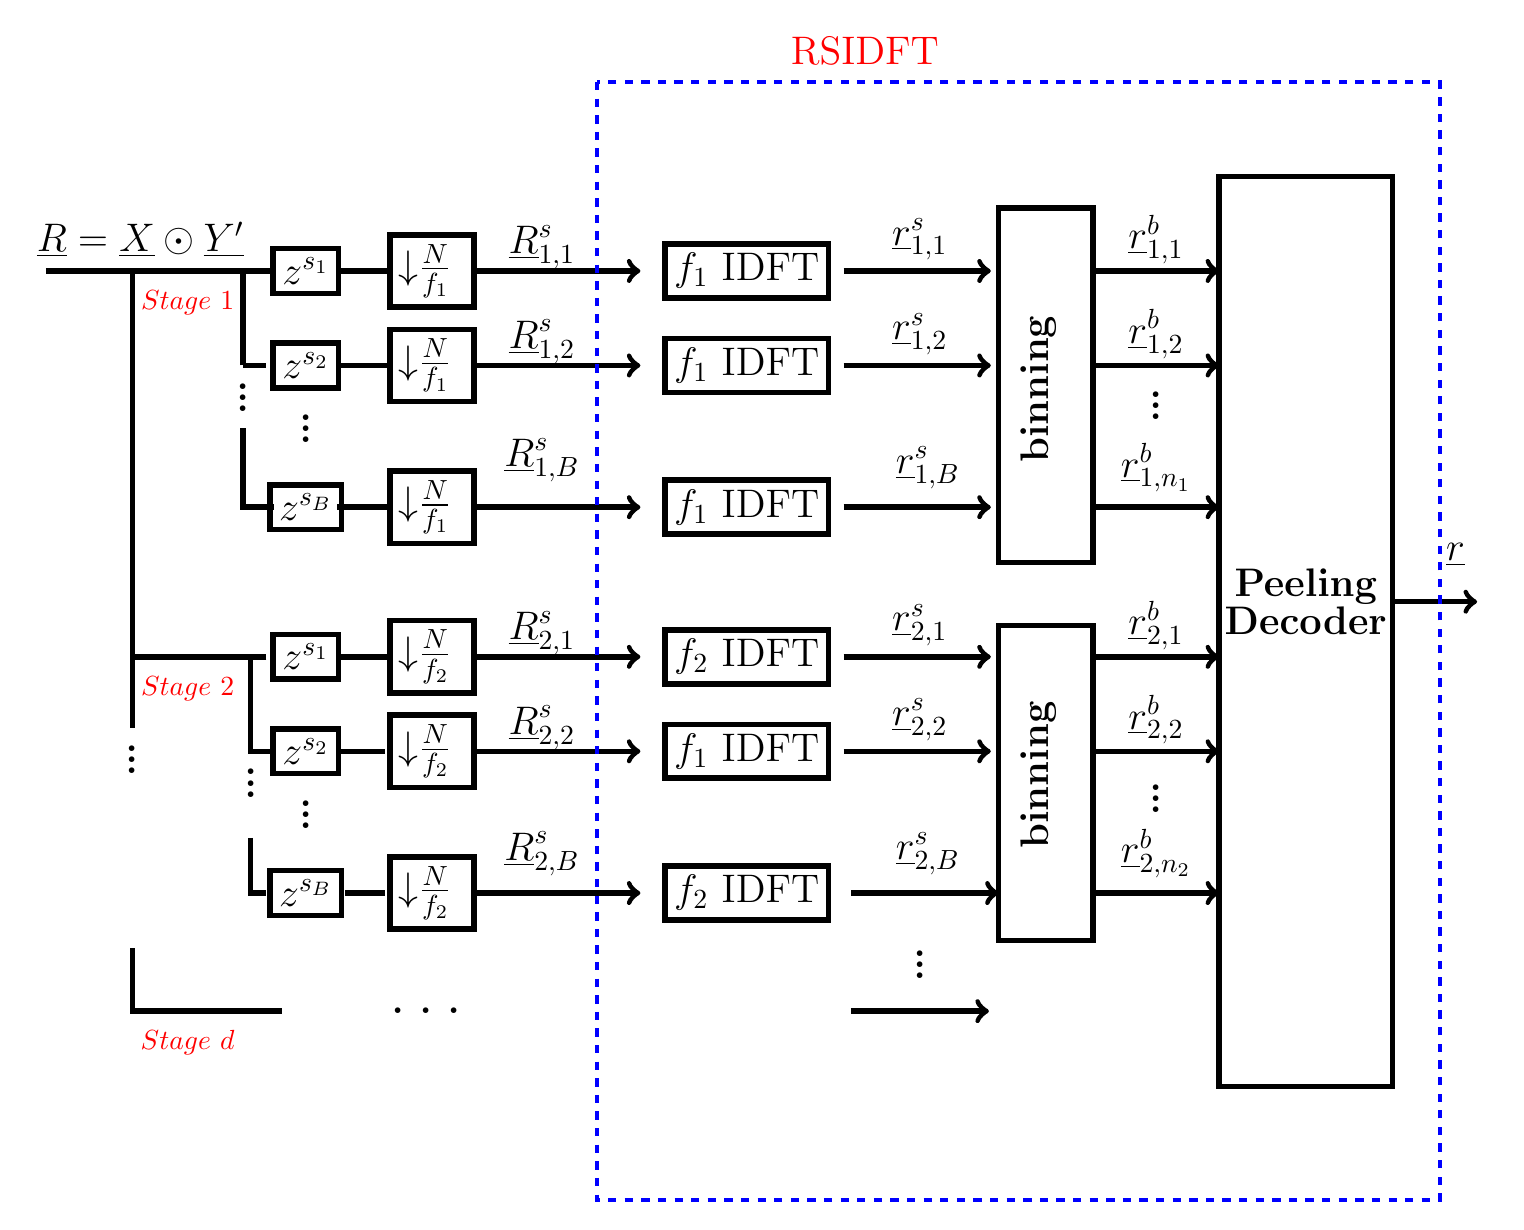
\begin{tikzpicture}

 % Downsampling blocks
\node[draw,align=center,thick,line  width =2pt] at (1.8,4.5) {\Large{$\mathbf{\downarrow} \frac{N}{f_2}$} };
\node[draw,align=center,thick,line  width =2pt] at (1.8,5.7) {\Large{$\mathbf{\downarrow} \frac{N}{f_2}$ }};
\node[draw,align=center,thick,line  width =2pt] (v6) at (1.8,2.7) {\Large{$\mathbf{\downarrow} \frac{N}{f_2}$ }};

\node[draw,align=center,thick,line  width =2pt] at (1.8,9.4) {\Large{$\mathbf{\downarrow} \frac{N}{f_1}$} };
\node[draw,align=center,thick,line  width =2pt] at (1.8,10.6) {\Large{$\mathbf{\downarrow} \frac{N}{f_1}$ }};
\node[draw,align=center,thick,line  width =2pt] at (1.8,7.6) {\Large{$\mathbf{\downarrow} \frac{N}{f_1}$ }};

%  Input lines to the down-sampling block

%  Delay blocks
\node[draw,align=center,thick,line  width =2pt] at (0.2,10.6) {\bf \Large{$z^{s_1}$}};
\node[draw,align=center,thick,line  width =2pt] at (0.2,9.4) {\bf \Large{$z^{s_2}$}};
\node[draw,align=center,thick,line  width =2pt] at (0.2,7.6) {\bf \Large{$z^{s_B}$}};

\node[draw,align=center,thick,line  width =2pt] at (0.2,5.7) {\bf \Large{$z^{s_1}$}};
\node[draw,align=center,thick,line  width =2pt] at (0.2,4.5) {\bf \Large{$z^{s_2}$}};
\node[draw,align=center,thick,line  width =2pt] at (0.2,2.7) {\bf \Large{$z^{s_B}$}};


% paths connecting the delay blocks  
 
 \draw[thick,line  width =2pt] (1.3,9.4) -- (0.6,9.4);
 

\node[line  width =2pt] at (-0.6,9.1) {\Huge{\vdots}};
\node[line  width =2pt] at (0.2,8.7) {\Huge{\vdots}};
\node[line  width =2pt] at (-0.5,4.2) {\Huge{\vdots}};
\node[line  width =2pt] at (0.2,3.8) {\Huge{\vdots}};

 \draw[thick,line  width =2pt] (1.3,10.6) -- (0.6,10.6);
 \draw[thick,line  width =2pt] (-0.6,9.4) -- (-0.6,10.6);
 
% paths connecting the two stages   
 \draw[thick,line  width =2pt] (-0.2,10.6) -- (-2,10.6);
 \draw[thick,line  width =2pt] (-0.6,9.4) -- (-0.3,9.4);
 \draw[thick,line  width =2pt] (-0.3,5.7) -- (-2,5.7);
 \draw[thick,line  width =2pt] (-2,5.7) -- (-2,10.6);
  \draw[thick,line  width =2pt] (-3.1,10.6) -- (-2,10.6);
  \draw[thick,line  width =2pt] (-2,5.7) -- (-2,4.8);
  
  
  % DFT blocks
\node[draw,align=center,thick,line  width =2pt] at (5.8,4.5) {\Large{$f_1$ IDFT}};
\node[draw,align=center,thick,line  width =2pt] at (5.8,5.7) {\Large{$f_2$ IDFT}};
\node[draw,align=center,thick,line  width =2pt] at (5.8,2.7) {\Large{$f_2$ IDFT}};

\node[draw,align=center,thick,line  width =2pt] at (5.8,9.4) {\Large{$f_1$ IDFT}};
\node[draw,align=center,thick,line  width =2pt] at (5.8,10.6) {\Large{$f_1$ IDFT}};
\node[draw,align=center,thick,line  width =2pt] at (5.8,7.6) {\Large{$f_1$ IDFT}};
% Connectors
 \draw[->,thick,line  width =2pt] (2.35,10.6) -- (4.45,10.6);
 \draw[->,thick,line  width =2pt] (2.35,9.4) -- (4.45,9.4);
 \draw[->,thick,line  width =2pt] (2.35,7.6) -- (4.45,7.6);
 
 \draw[->,thick,line  width =2pt] (2.35,5.7) -- (4.45,5.7);
 \draw[->,thick,line  width =2pt] (2.35,4.5) -- (4.45,4.5);
 \draw[->,thick,line  width =2pt] (2.35,2.7) -- (4.45,2.7);

 \draw[->,thick,line  width =2pt] (10.23,10.6) -- (11.8,10.6);
 \draw[->,thick,line  width =2pt] (10.23,9.4) -- (11.8,9.4);
 \draw[->,thick,line  width =2pt] (10.23,7.6) -- (11.8,7.6);
 
 \draw[->,thick,line  width =2pt] (10.23,5.7) -- (11.8,5.7);
 \draw[->,thick,line  width =2pt] (10.23,4.5) -- (11.8,4.5);
 \draw[->,thick,line  width =2pt] (10.23,2.7) -- (11.8,2.7);
 
  \draw[->,thick,line  width =2pt] (7.03,10.6) -- (8.9,10.6);
 \draw[->,thick,line  width =2pt] (7.03,9.4) -- (8.9,9.4);
 \draw[->,thick,line  width =2pt] (7.03,7.6) -- (8.9,7.6);
 
 \draw[->,thick,line  width =2pt] (7.03,5.7) -- (8.9,5.7);
 \draw[->,thick,line  width =2pt] (7.03,4.5) -- (8.9,4.5);
 \draw[->,thick,line  width =2pt] (7.13,2.7) -- (9,2.7);
 
  % Labels
  \node[draw=none,align=center] at (-1.9,11) {\Large{$\underline{R}= \underline{X} \odot \underline{Y'}$}};
  
  \node[draw=none,align=center] at (3.2,10.9) {\Large{$\underline{R}^{s}_{1,1}$}};
  \node[draw=none,align=center] at (3.2,9.7) {\Large{$\underline{R}^{s}_{1,2}$}};
\node[draw=none,align=center] at (3.2,8.2) {\Large{$\underline{R}^{s}_{1,B}$}};

\node[draw=none,align=center] at (3.2,6) {\Large{$\underline{R}^{s}_{2,1}$}};
  \node[draw=none,align=center] at (3.2,4.8) {\Large{$\underline{R}^{s}_{2,2}$}};
  \node[draw=none,align=center] at (3.2,3.2) {\Large{$\underline{R}^{s}_{2,B}$}};

  \node[draw=none,align=center] at (8,11) {\Large{$\underline{r}^{s}_{1,1}$}};
  \node[draw=none,align=center] at (8,9.8) {\Large{$\underline{r}^{s}_{1,2}$}};
  \node[draw=none,align=center] at (8.1,8.1) {\Large{$\underline{r}^{s}_{1,B}$}};
  
    \node[draw=none,align=center] at (11,11) {\Large{$\underline{r}^{b}_{1,1}$}};
  \node[draw=none,align=center] at (11,9.8) {\Large{$\underline{r}^{b}_{1,2}$}};
  \node[draw=none,align=center] at (11,8.1) {\Large{$\underline{r}^{b}_{1,n_1}$}};
  
     \node [draw=none] at (11,9) {\Huge{\vdots}} ;
   
  \node[draw=none,align=center] at (8,6.1) {\Large{$\underline{r}^{s}_{2,1}$}};
  \node[draw=none,align=center] at (8,4.9) {\Large{$\underline{r}^{s}_{2,2}$}};
  \node[draw=none,align=center] at (8.1,3.2) {\Large{$\underline{r}^{s}_{2,B}$}};
  
  \node [draw=none] at (11,4) {\Huge{\vdots}} ;
  
    \node[draw=none,align=center] at (11,6.1) {\Large{$\underline{r}^{b}_{2,1}$}};
  \node[draw=none,align=center] at (11,4.9) {\Large{$\underline{r}^{b}_{2,2}$}};
  \node[draw=none,align=center] at (11,3.2) {\Large{$\underline{r}^{b}_{2,n_2}$}};
  
  \node [draw=none] at (-2,4.5) {\Huge{\vdots}} ;
  
   \node[draw=none,align=center] at (-1.3,10.2) {\color{red}$Stage ~1$};
  \node[draw=none,align=center] at (-1.3,5.3) {\color{red}$Stage ~2$};
   \node[draw=none,align=center] at (-1.3,0.8) {\color{red}$Stage ~d$};
\draw [thick,line  width =2pt](-2,2) -- (-2,1.2) -- (-0.1,1.2) ;
 \node[draw=none,align=center] at (1.8,1.2) {\Huge{\ldots}};
 
\draw [thick,line  width =2pt] (11.8,0.2424) rectangle (14,11.8);
\node (v1) at (7,1.2) {};
\node (v2) at (9,1.2) {};



\node (v11) at (1.3,7.6) {};


\draw  [->,thick,line  width =2pt](v1) edge (v2);
\node at (8,1.9) {\Huge{\vdots}};
\node [text width=3cm, align =center ] at (12.9,6.4) {\Large \bf Peeling \\ Decoder};
\node (v3) at (13.9,6.4) {};
\node (v4) at (15.2,6.4) {};
\draw [thick, ->,line  width =2pt] (v3) edge (v4);
\node at (14.8,7) {\Large{$\underline{r}$}};

\draw[thick,line  width =2pt] (-0.6,8.6) -- (-0.6,7.6) -- (-0.2,7.6);
\draw[thick,line  width =2pt] (0.6,7.6) -- (1.3,7.6);
\draw[thick,line  width =2pt] (-0.5,5.7) -- (-0.5,4.5) -- (-0.2,4.5);
\draw[thick,line  width =2pt] (-0.5,3.4) -- (-0.5,2.7) -- (-0.3,2.7);
\draw [thick,line  width =2pt](0.6,5.7) -- (1.3,5.7);
\draw[thick,line  width =2pt] (0.6,4.5) -- (1.2,4.5);
\draw[thick,line  width =2pt] (0.7,2.7) -- (1.2,2.7);
\draw [dashed, color=blue, line width =1.5pt ] (3.9,13) rectangle (14.6,-1.2);
\node[color =red] at (7.3,13.4) {\Large RSIDFT  };
\draw [thick, line width =2pt]  (9,11.4) rectangle (10.2,6.9);
\draw [thick, line width =2pt]  (9,6.1) rectangle (10.2,2.1);
\node[rotate=90] at (9.5,9.1) {\Large \bf binning};
\node[rotate=90] at (9.5,4.2) {\Large \bf binning};
\end{tikzpicture}